\documentclass[final_report.tex]{subfiles}

\begin{document}

\section{Design Considerations}
\label{sec:design}

\subsection{Data Sharing}
The proposed application will be sharing data between the DPDK code written in C (low level) and the Java (medium level) side used for the highly abstracted part of the application. This requires a large amount of data, most noticeably packets, to be transferred between 'sides' in a small amount of time. This section will explore possible techniques for this data sharing, discuss the advantages and disadvantages and finally reason about a decision.

\subsubsection{Memory Usage}
Programs written in most languages make use of memory on heap, off heap and in a stack. Stack memory is used for local, short term variables which this report isn't concerned with. Heap memory is a block of memory associated with a program for it to store long lasting data on which can be shared among multiple threads. Some languages require allocation of data on heap memory to be freed.

Within Java, heap memory is subjected to a garbage collector which scans the heap when the JVM is running out of memory and dereferences any objects which aren't in use any more while compact the heap by moving references around. Although memory management is taken away from the user, the garbage collector can slow down an application as it traverses memory at random intervals. Off heap memory isn't subjected to the garbage collector which allows fast processing applications to take advantage of this while memory can be referenced directly.

The application needs to assign memory efficiently to have any chance of fast performance. Figure \ref{fig:pipeline} shows the problem which needs to be overcome using memory management with different techniques. The data will follow a pipeline flow, starting on the NIC receive queue and been retrieved as a Mbuf struct containing all of the packet data. From there a 'technique' needs to be implemented to efficiently map the data in the struct to a Java packet object. The data will then be processed depending on the application requirements and then will be forwarded via been put on the transmit queue of the NIC. Between these stages, the data needs to be mapped back from the Java object to the original struct using a 'technique'

There are a number of possible 'techniques' available in order pass data efficiently between native structs and Java objects. The implementations are discussed below along with the advantages and disadvantages.

\begin{figure}[H]
	\centering
	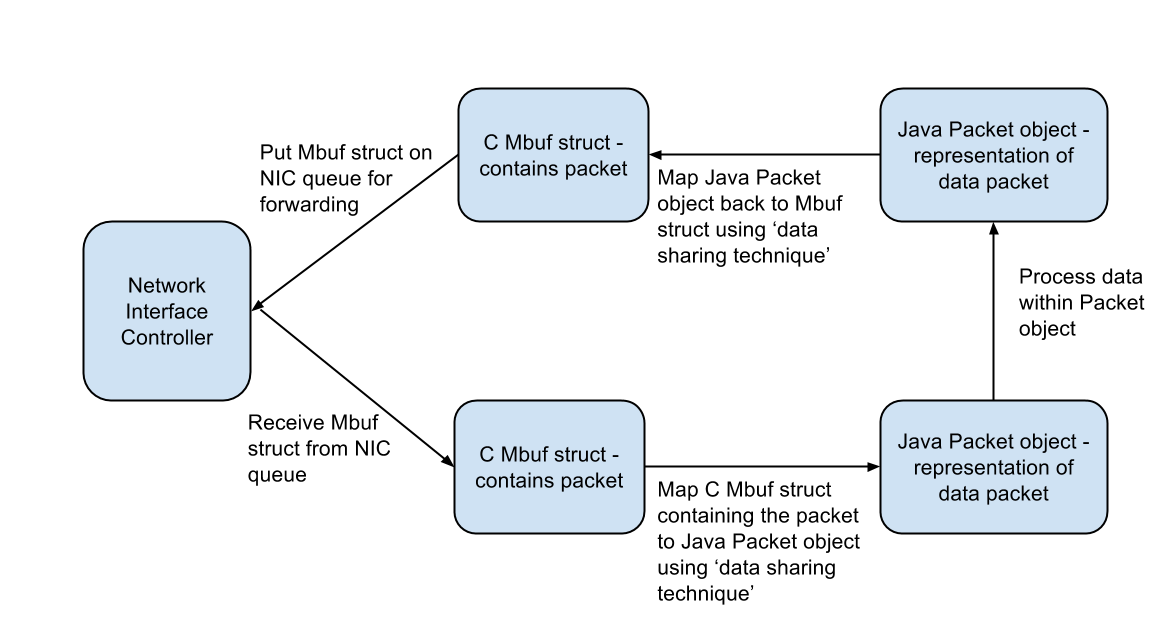
\includegraphics[width=0.8\textwidth]{img/pipeline.png}
	\caption{Server}
	\label{fig:pipeline}
\end{figure}

\subsubsection{Objects and JNI}
By far the simplest technique available is using the Java Native Interface (JNI) in order to interact with native code and then retrieve the required data via object method accessing provided by the JNI environment pointer. This can be done 2 ways, either by creating the object and passing it as a parameter to the native methods or creating an object on the native side. Both ways require the population of the fields to be done on the native side. From then on, any data manipulation and processing could be done on the Java side. Unfortunately, this does require all data to be taken from the object and placed back into the structs before packets can be forwarded. Obviously this results in a lot of unneeded data copying, while the actual JNI calls can significantly reduce the speed of the application as shown in \todo{ref this}.

There are a few frameworks which aim to solve the problem of mapping structs to objects while trying to increase the overall speed of the JNI using different techniques.

\paragraph*{Java Native Access (JNA)}
The JNA is a community developed framework which aims to abstract the JNI and native code away from developers who want to use native shared libraries. It uses its own data mapping between native and Java data types with automatic conversion of string and object to character arrays and structs. Although this framework provides much of the functionality within this project, it focusses on correctness and ease of use and therefore neglects performance.

\paragraph*{Javolution}
Javolution is similar to the JNA but focusses more on real-time performance within Java. It provides a number of high performance utilities for this purpose while allowing access to native libraries. For this purpose, struct and union classes are created automatically for mapping between objects. Javolution provides the functionality required for this project but it requires a lot initial set-up which can be heavy, especially for small applications like middleboxes.

\paragraph*{Swig}
Simplified Wrapper and Interface Generator(Swig) differs from JNA and Javolution simply because the framework only focusses on object and struct mapping. It abstracts all creation of objects, structs, access methods and memory allocation away from the user via an interface. Although very useful, it lacks performance when handling numerous objects in quick succession. 

\subsubsection{Byte Buffers}
Byte buffers are a Java class which allow for memory to be allocated on the Java heap (non direct) or outside of the JVM off heap (direct), while abstracting pointer arithmetic and boundary checks away from the application. Non direct byte buffers are simply a wrapper for a byte array on the heap and are generally used as they allow easier access to the data as multiple byte reading and data type conversion is handled by the class. Direct byte buffers allocate memory outside of the JVM in native memory which means that the only limit on the size of byte buffers is memory itself.

The performance characteristics of direct and non-direct byte buffers are very similar. Direct byte buffers can be improved by aligning the bytes with the native endian (normally little endian) format since the class makes use of the Java Unsafe native access which allows for the methods to be in-lined with machine code.

The Java garbage collector doesn't have access to native memory and therefore direct byte buffers allow the application to manage memory and reduce memory usage. Garbage collection bottlenecks within high performance system are therefore reduced. For direct byte buffers, the actual object is stored on the heap and but the memory banks are off heap meaning that the pointer to the memory bank will not change, even if the byte buffer objects gets moved around by the garbage collector. This can be vital as it allows direct referencing of the memory for quicker data access.

Direct byte buffers would be an ideal choice for data sharing if it was possible to redirect DPDK mbuf structs onto the byte buffer directly, consequently allowing the Java side easy access to the data using the byte buffer API. However, since DPDK makes use of huge pages and handles its own memory management, it's not possible to use byte buffers directly as the memory for the NIC queues. Instead, data would have to be copied from structs and extracted into objects and vice versa.

\subsubsection{Java Unsafe}
The Java Unsafe class is actually only used internally by Java for its memory management. It generally shouldn't be used within Java since it makes a safe programming language like Java an unsafe language (hence the name) since memory access exceptions can be thrown which will ultimately crash the JVM. Even so, it has a number of uses such as:

\paragraph*{Object initialisation skipping}
This is where any instance of an object can be created from the class, but no constructors are used meaning that the object created without any of the fields set. This has a number of uses including security check bypassing, creating instances of objects which don't have a public constructor and allowing multiple objects of a singleton class.

\paragraph*{Intentional memory corruption}
This allows the setting of private fields of any object. It is a common way of bypassing security features as private fields to allow access to certain situation can be overwritten to gain access.

\paragraph*{Nullifying unwanted objects}
This has a common use of nullifying passwords after they have been stored as strings. If a password is stored as a string in Java, even setting the field to \textit(null) will only dereference it. The original string will still be in memory after the dereferencing up until it is garbage collected. Even rewriting the field with a new field won't work as strings are immutable in Java. This makes it susceptible to a timing attack to retrieve the password. Using unsafe allows for the actual memory location to be overwritten with random values to prevent this.

\paragraph*{Multiple inheritance}
Java doesn't allow multiple inheritance within its class declaration of casting. However, using Unsafe any object can be cast to any other object without a compiler of run-time error. This obviously only works if data fields are compliant with each other and any method invocations are referenced. 

\paragraph*{Very fast serialization}
The Java \textit{Serializable} abstraction is well known to be slow, which can be a major bottleneck in fast processing applications over a network. Even the \textit{Externalizable} functionality isn't much factor and that requires an class schema to be defined. However, custom serializing can be extremely fast using the Unsafe Class. Basically allocating memory and then putting/getting data from the memory requires little JVM usage and can be done with machine instructions.

Obviously without proper precautions any of these actions can be dangerous and can result in crashing the full JVM. This is why the Unsafe class has a private constructor and calling the static Unsage.getUnsafe() will throw a security exception for untrusted code which is hard to bypass. Fortunately, Unsafe has its own instance called 'theUnsafe' which can be accessed by using Java reflection:

\begin{lstlisting}[language=Java, caption={Accessing Java Unsafe}, label=lst:java_unsafe]
Field f = Unsafe.class.getDeclaredField("theUnsafe");
f.setAccessible(true);
Unsafe unsafe = (Unsafe) f.get(null);
\end{lstlisting}

Using Unsafe then allows direct native memory access (off heap) to retrieve data in any of the primitive data formats. Custom objects with a set structure can then be created, accessed and altered using Unsafe which provides a vast increase in performance over traditional objects stored on the heap. This is mainly thanks to the JIT compiler which can use machine code more efficiently by in-lining certain memory access directly with assembly code. This also removes the need for copying of data between memory locations, structs and objects, therefore meaning it is zero-copy.

\subsection{Packing Structures}
Structures (structs) are a way of defining complex data into a grouped set in order to make this data easier to access and reference as shown in Code \ref{lst:c_struct}. They are heavily used with C applications and can be seen as Java object without the associated methods.

\begin{lstlisting}[language=C, caption={Example C Struct}, label=lst:c_struct]
struct example {
    char *p;
    char c;
    long x;
    char y[50];
    int z;
};
\end{lstlisting}

On modern processors all commercially available C compilers will arrange basic C data types in a constrained order to make memory access faster. This has 2 effects on the program. Firstly, all structs will actually have a memory size larger than the combined size of the data types in the struct as a result of padding. However, this generally is a benefit to most consumers as this memory alignment results in a faster performance when accessing the data.

\todo[inline]{Explain why it has faster performance}
\todo[inline]{Nested padding in struct?}
\todo[inline]{C struct field always in given order}
\todo[inline]{Inconsistencies with data type length so using uint32t etc}

Code \ref{lst:c_padded_struct} shows a struct which has compiler inserted padding. Any user wouldn't know the padding was there and wouldn't be able to access the data in the bits of the padding through conventional C dereferencing paradigm (only via pointer arithmetic). This example does assume use on a 64-bit machine with 8 byte alignment, but 32-bit machines or a different compiler may have different alignment rules.

\begin{lstlisting}[language=C, caption={Example C Struct with compiler inserted padding}, label=lst:c_padded_struct]
struct example {
    char *p;       // 8 bytes
    char c;        // 1 byte
    char pad[7];   // 7 byte padding
    short x;       // 2 bytes
    char pad[6];   // 6 byte padding
    char y[50];    // 50 bytes
    int z;         // 4 bytes
};
\end{lstlisting}
\todo[inline]{Mention this is on 64-bit machine and obviously you don't notice padding and order of elements can pay an important part in this}

\begin{lstlisting}[language=C, caption={Example C Struct stopping padding}, label=lst:c_packed_struct]
struct __attribute__((__packed__)) example {
    char *p;       // 8 bytes
    char c;        // 1 byte
    short x;       // 2 bytes
    char y[50];    // 50 bytes
    int z;         // 4 bytes
};
\end{lstlisting}

Since the proposed application in this report requires high throughput of data, the initial thought would be that this optimisation is a benefit to the program. Generally this is the case, but for data which is likely to be shared between the C side and Java side a large amount, data accessing is far quicker \todo{Proof on speed} on the Java side if the struct is packed (no padding). This results in certain structs been forced to be packed when compiled, more noticeably, those used for packet and protocol headers.

Packed structures mean there are no gaps between elements, required alignment is set to 1 byte. Also \_\_attribute\_\_((packed)) definition means that compiler will deal with accessing members which may get misaligned due to 1 byte alignment and packing so reading and writing is correct. However, compilers will only deal with this misalignment if structs are accessed via direct access. Using a pointer to a packed struct member (and therefore pointer arithmetic) can result in the wrong value for the dereferenced pointer. This is since certain members may not be aligned to 1 byte. In the below example, unint32 is 4 byte aligned and therefore it is possible for a pointer to it to expect 4 byte alignment therefore resulting in the wrong results.

\begin{lstlisting}[language=C, caption={Example C Struct with compiler inserted padding}, label=lst:c_padded_struct]
#include <stdio.h>
#include <inttypes.h>
#include <arpa/inet.h>

struct packet {
    uint8_t x;
    uint32_t y;
} __attribute__((packed));

int main ()
{
    uint8_t bytes[5] = {1, 0, 0, 0, 2};
    struct packet *p = (struct packet *)bytes;

    // compiler handles misalignment because it knows that
    // "struct packet" is packed
    printf("y=%"PRIX32", ", ntohl(p->y));

    // compiler does not handle misalignment - py does not inherit
    // the packed attribute
    uint32_t *py = &p->y;
    printf("*py=%"PRIX32"\n", ntohl(*py));
    return 0;
}
\end{lstlisting}

On an x86 system (which does not enforce memory access alignment), this will give y=2 and *py=2 which is as expected. Conversely, other systems using the SPARC architecture or similar will give y=2 and *py=1 which isn't what the user would expect.

However, since a packed struct is much easier to traverse from Java than a padded struct, the decision was made to make certain structs packed within the DPDK framework and then recompile the libraries. This decision could be made since other structs within the DPDK framework were also packed and therefore consideration of this was already made.

Note that if a struct contains another struct, that struct should be packed recursively as-well to ensure the first struct has no padding at all.

Char doesn't have alignment and can start on any address. But 2-byte shorts must start on an even address, 4-byte integers or floats must start on an address divisible by 4, and 8-byte longs or doubles must start on an address divisible by 8. Signed or unsigned makes no difference.

Self-alignment makes access faster because it facilitates generating single-instruction fetches and puts of the typed data. Without alignment constraints, on the other hand, the code might end up having to do two or more accesses spanning machine-word boundaries. Characters are a special case; they're equally expensive from anywhere they live inside a single machine word. That's why they don't have a preferred alignment.

Casting to an odd pointer will slow down code and could work. Other architectures will take the word which the pointer points to and therefore the problem occurs above.

\subsection{Performance testing}
In order to evaluate the most suitable data sharing technique, performance testing on 4 different implementation options for sharing data between Java and native memory were considered. Since the ultimate aim of the implementation is to maximise throughput of packets, the performance test tried to mimic this by processing data on 1 million packets per iteration. This processing involved retrieving data from the native packet struct, loading that data into a Java object, changing the data and then setting the data back into the original struct. Various techniques to do this were used to try and find the best performance possible. All of the techniques made use of a static native struct which acted like a new packet been received. The changed data was then set back into this struct.

\begin{algorithm}[H]
	\caption{Data Sharing Performance Test Algorithm}
	\label{alg:data}
	\begin{algorithmic}[1]
		\Function{Main}{}
			\For{i = 1 to 10}
				\State startTimer
				\State \Call{performTest}{ }
				\State stopTimer
				\State outputTime				
			\EndFor
		\EndFunction
		\newline
		\Function{performTest}{}
			\For{i = 1 to 1000000}
				\State retreiveData
				\State setNewData
				\State saveData
			\EndFor
		\EndFunction
	\end{algorithmic}
\end{algorithm}

Considering there were 4 different data sharing techniques tested, the \textit{retrieveData}, \textit{setNewData} and \textit{saveData} methods were different and are described below:

\paragraph*{Object Passing}
The object technique involved creating a packet and sending its reference through the JNI to the native code. From there, this packet could be populated with data from a given struct through the Java environment pointer. For each setter method called, the method id of that method must be retrieved for the given class so the combination of that and the packet reference could set the data.

From there, new data is input into the packet from the Java side and passed back through to JNI so the struct can be set with the new data. This is done using getters for the objects' fields via the Java environment pointer.

\paragraph*{Byte Buffer}
The technique involved declaring a direct byte buffer to assign off heap memory of the size of the packet struct. From there, the pointer to this memory location was sent to the native code, where data from the struct was directly copied into the byte buffer, therefore populating the byte buffer with duplicate data. The Java code then pulled the data from this via the byte buffer's inbuilt methods and set the data into a new packet object. From there the packet object could be used whenever desired.

To save the data back into the original struct, the data was copied from the packet object back into the byte buffer in the order of the members of the struct. The data was then pulled from the memory of the byte buffer and set back into the original struct.

\paragraph*{Unsafe}
Using the Unsafe class allows for direct access to members of the struct. To take account for this this technique first allocates off heap memory for the pointer to the struct to be stored. This pointer is put into the memory location natively and accessed via Unsafe methods. From this, data can be accessed directly from the struct and input to a new packet object for later use. New data is then set in the object.

To set the data in the struct, the data is removed from the object and directly put into the struct. This is done using the pointer and the correct byte offsets depending on the previous data type entered.

\paragraph*{Direct}
Direct accessing relates to not storing the struct members in Java at all. Instead a different type of Packet object is used which just stores pointers to the struct. From there any accessing and setting of data is simply done using the Unsafe class to directly get or set the values within the struct. This different packet object also contains offset information for the struct so the correct values are accessed.

\subsubsection{Expectations}
Of the 4 techniques, it is expected that the object method would be by far the slowest, mainly due to the excessive number of JNI calls used which significantly slows an application down. The Byte Buffer method will most likely be the slowest of the other 2 techniques due to the large number of data copying which goes on. The other 2 techniques (unsafe and direct) will likely be very close in performance, mainly because they both use direct accessing into the struct. The unsafe technique should be slightly slower however due to the setting and getting from the packet object.

\todo{evaluate each technique on ease and number of data copies and results and say why we picked 1 of the others}

\subsubsection{Results}
The graphs in figures \ref{fig:res1}, \ref{fig:res2} \& \ref{fig:res3} show the results from the different techniques run on different systems. Considering there were 10 iterations of 1 million packets per technique the results show the averages of the times. However, certain times were disregard and seen as anomalies since they were well above the average \todo{stats for this}. These readings were generally the initial values after the 1st iteration and can be either be related to the just in time compiler warming up after switching to a different class or garbage collection on the vast number of objects left over from the previous technique.

The graphs show the time in nanoseconds which it took to process an individual packet, but the scale is logarithmic due to the excessive size of the object technique. For easier reading, the numbers at the top of the columns show the times factor for each technique compared to the fastest. For example, on Figure \ref{fig:res1} the byte buffer takes 2.74 times the direct technique to process the packet.

\begin{figure}[H]
	\centering
	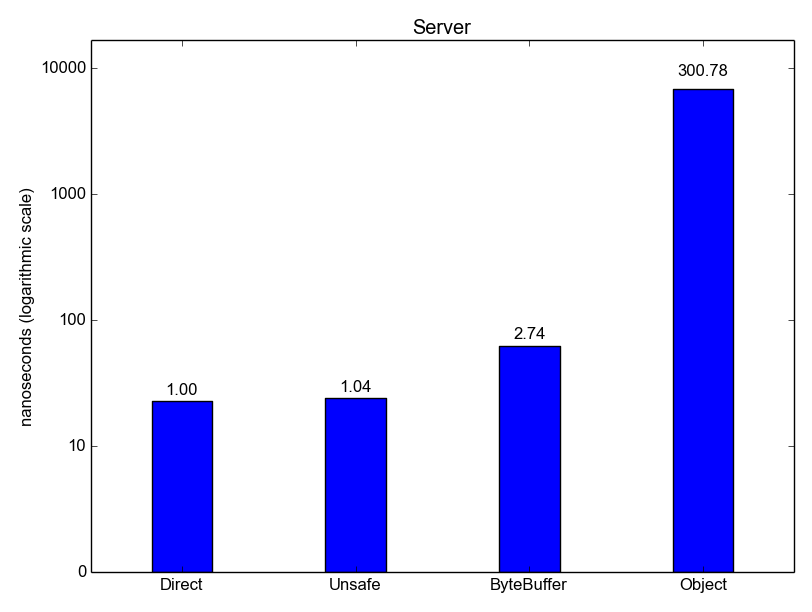
\includegraphics[width=0.8\textwidth]{img/server.png}
	\caption{Linux - Intel Xeo E5-2690 at 2.90GHz with 32 cores}
	\label{fig:res1}
\end{figure}

\begin{figure}[H]
	\centering
	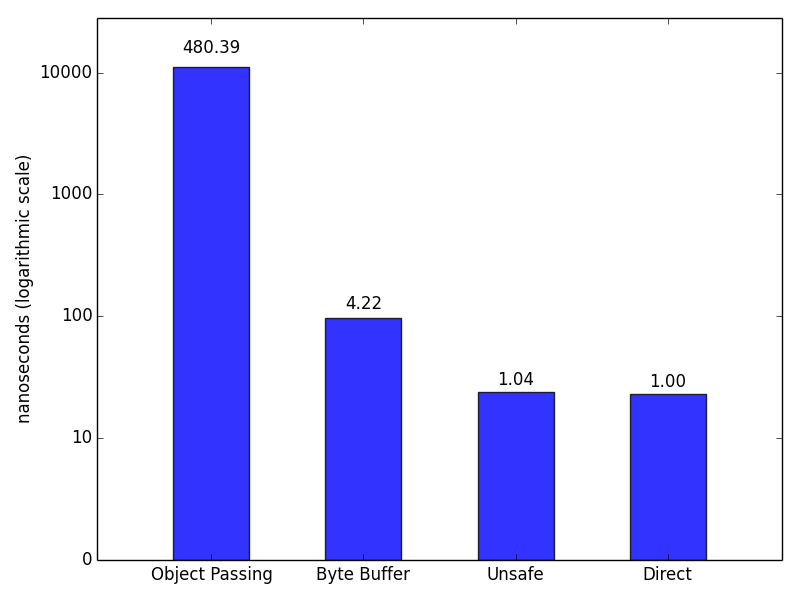
\includegraphics[width=0.8\textwidth]{img/mac.png}
	\caption{Mac OS X - Intel i7-3615QM at 2.30GHz with 8 cores}
	\label{fig:res2}
\end{figure}

\begin{figure}[H]
	\centering
	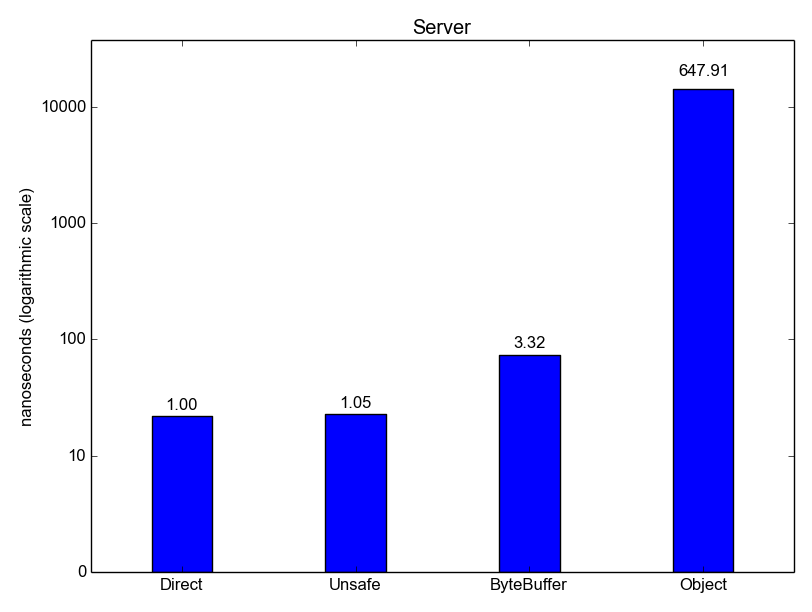
\includegraphics[width=0.8\textwidth]{img/vm.png}
	\caption{Linux VM on Mac OS X - Intel i7-3615QM at 2.30GHz with 4 cores}
	\label{fig:res3}
\end{figure}

\subsubsection{Evaluation}
As the graphs show, the exceptions declared earlier have been met. The object technique should be completely disregard, even though it offers the easiest solution. Due to its abysmal performance, been 300 - 650 times slower than the faster technique, its not going to help with packet throughput.

For similar reasons Byte buffer should be disregarded as well simply because its too slow compared to the other methods. The amount of data copying with this technique is the downfall, although this could have potentially worked if structs could be directly written into the buffers. \todo{cant be done and reference earlier}

The difference between the direct and unsafe methods is minimal on all 3 machines. The direct technique is slightly faster since it doesn't copy the data into the object although Java is surprisingly fast at this as proven by the unsafe results. Furthermore, in general middleware software, there isn't the requirement to access all data fields of the packets generally, therefore storing them all in objects can be seen as needless copying. This is where the direct access technique excels since it only accesses data which it needs to been zero-copy. Direct access was therefore chosen as the technique to use for the implementation which goes into further details about how this was done.

\subsection{Thread affinity}
Normally as a thread gets a time slice (a period in which to use the core), it is granted whichever core is determined to be most free by the operating system's scheduler. However, due to the scheduler and context switching of threads, a thread may move around a number of different cores during its execution cycle.

Thread affinity aims to reduce this context switching which can be expensive, by limiting threads to 1 or a subset of the available cores. Even if the thread is scheduled to have a 'break', since it doesn't change cores there is no need to copy data between core caches which ultimately improves performance. 

Therefore, for primarily single (or limited) thread applications, it is sometimes best to set the CPU affinity to a specific core, or subset of cores. This will allow the 'Turbo' processor frequency scaling to kick in and be sustained (instead of skipping around to various cores that may not be scaled up, and could even be scaled down).

\begin{lstlisting}[language=C, caption={Example of setting thread affinity}, label=lst:c_affinity]
cpu_set_t cpuset;	\\ structure used to manage cpu affinity settings
pthread_t thread = pthread_self();  \\ get own system wide thread id
CPU_ZERO(&cpuset); \\ zero cpuset structure
CPU_SET(5, &cpuset); \\ set cpuset structure use with the 6th core (0-5)
int res = pthread_setaffinity_np(thread, sizeof(cpu_set_t), &cpuset); \\ set affinity of thread
\\ error handling here of res
res = pthread_getaffinity_np(thread, sizeof(cpu_set_t), &cpuset); \\ check affinity of thread
\\ error handling here of res
\end{lstlisting}
\todo{ref this}

In Linux, Java threads uses the native thread(i.e, thread provided by Linux which is normally the POSIX thread). This means the JVM creates a new native thread when the Java code creates a new Java thread. Java provides access to the thread which is currently running via the \textit{Thread.currentThread().getId()} call but this actually only gets the JVMs id number of the thread which is local. For affinity threading to be set the system thread id us required.

Since the Java standard library does not provide functionality for affinity threading, then this function need to be provided through custom native methods. A native thread can be bound to a core through the pthread\_setaffinity\_np() function. Code \ref{lst:c_affinity} shows the basic steps of how to achieve affinity threading.

\begin{figure}[H]
	\centering
	\begin{subfigure}{0.5\textwidth}
		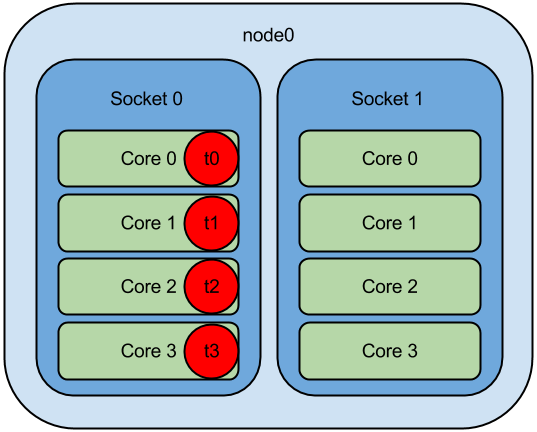
\includegraphics[width=\textwidth]{img/aff1.png}
		\caption{Compact scheduling}
		\label{fig:aff1}
	\end{subfigure}%
	\begin{subfigure}{0.5\textwidth}
		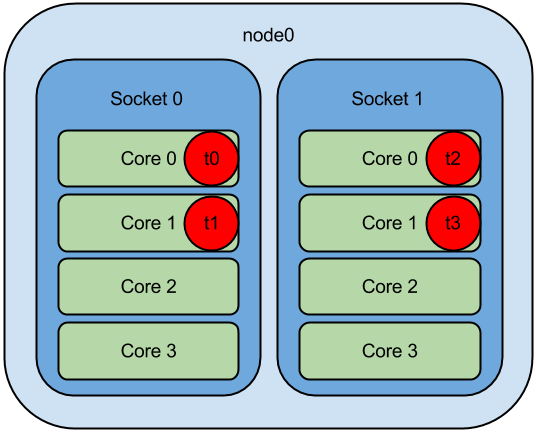
\includegraphics[width=\textwidth]{img/aff2.png}
		\caption{Round robin scheduling}
		\label{fig:aff2}
	\end{subfigure}
	\caption{Scheduling concerns of threads on cores with multiple sockets}
	\label{fig:aff}
\end{figure}

For the implementation of affinity threads, a few further considerations need to be undertaken concerning the assignment of cores depending on the number of sockets. If there is only 1 processor socket, there is no problem, but when there are multiple sockets consideration about the thread layout on the sockets becomes vital.

Figure \ref{fig:aff} shows potential layouts for threads. Compact scheduling (figure \ref{fig:aff1}) is primarily used when threads are sharing data and therefore accessing the same NUMA memory, as accessing data between sockets is relatively slow. Round robin scheduling (figure \ref{fig:aff2}) benefits from quicker memory access as its shared between fewer active cores. This can lead to increased performance but only works of the threads are independent of each other. For consideration needs to be taken into account for the socket layout of the NICs, as threads should be accessing queues on the same memory socket to increase performance.

\subsection{Endianness}
This describes the order in which bytes of data types are stored in memory relative to pointers. In big-endian systems, the most significant bytes are stored at the pointer with every successive data bytes stored in successive memory locations. Conversely, in little-endian systems, the least significant byte is stored at the pointer. There is no advantage or disadvantage to either endian types, its simply a matter on convention for certain systems. Figure \ref{fig:endian} shows how different endian systems store the value of the hexadecimal value \textit{0x0A0B0C0D}. 

\begin{figure}[H]
	\centering
	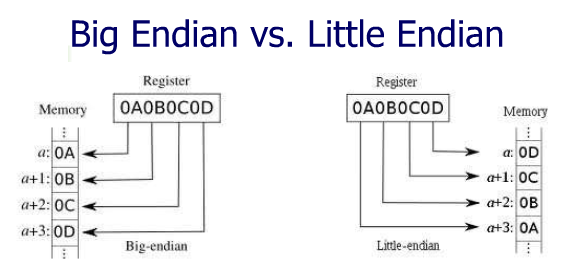
\includegraphics[width=\textwidth]{img/endian.png}
	\caption{Difference between little and big endian}
	\label{fig:endian}
\end{figure}

This becomes a problem when using the Java Native Interface with native code code on Intel architectures since the Java Virtual Machine uses big-endian format while Intel uses little-endian format. Normally the JNI environment would handle this byte ordering conversion but since the JNI has been proven to be too slow \todo{ref this} to meet the requirement, this needs to be handled by the application.

\subsection{Data type conversion}
Between different languages the same data type can be represented by varying lengths in bytes and whether unsigned or signed (in the case of numerical values). It can also be the case that data type lengths in native languages differ depending on the architecture and whether it is 32-bit or 64-bit.

This becomes more of an issue when sharing data between C and Java. Java always uses a signed integer representation with the most significant bit representing whether the number is negative or positive. C uses both signed and unsigned representation depending on the requirements with varying byte length. Again, any conversion between the differences is normally handled via the JNI, but since the implementation aims to bypass the JNI as much as possible, data type conversion will have to be handled.

Lets take the integer representation as an example. In C, and integer can vary between 2, 4 and 8 bytes in length depending on the architecture and compiler. To solve this, standard integer types are used (e.g. uint8\_t \& int32\_t) which guarantee that the representation is at least the length of the type definition stated. In Java, an integer is guaranteed to be 4 bytes long regardless of the system. However, DPDK uses unsigned integers while Java uses signed integers. This requires conversion between the unsigned and signed, but since unsigned has a higher upper bound on the value it can store due to the extra bit (MSB) there can be an overflow error when converting to Java. This requires that Java uses a long (8 byte) representation to hold the C 4 byte unsigned integer.

Conversion from Java to C then could then result in an underflow error if a value which can be represented by a Java long can't be represented by a C integer. This means bound checking is required on the Java side for any number conversions.

\todo{get a table of this}

\subsection{Protocol undertaking}
There are numerous protocols which need implementation in order to handle a full range of network traffic. However, since this report primarily focusses on the implementation and testing of basic middleboxes, many of these protocols will be neglected.

Only the layer 3 Internet Protocol (IP) will be supported and consequently so will the IPv4 and IPv6 packet headers. The User Datagram Protocol (UDP) and the transmission control protocol (TCP) for the 4th layer of the IP stack with be supported in terms packet checking for these headers. Actual inspection of the headers and the data will not be supported.

Furthermore, even though Address Resolution Protocol (ARP) is a fundamental part of the stack for Ethernet connection, this will not be supported and therefore RARP requests won't be either. By only taking a small subset of the available protocols it allows more focus to be aimed at the techniques of the implementation rather than the less interesting repetitive coding.

\subsection{Configuration Files}
DPDK takes a large number of user defined flags and values when starting the application via the command line to set up the EAL correctly. These flags can be further extended by the application to have their own specific variables. This can results in a lengthy start-up command which isn't easy to change on the fly.

For this reason, the implementation will use a different style of user defined variables. A 'properties' configuration file will instead be used to simply the application start-up allowing for configuration to be swapped in and out when required. These variables are as follows:

\begin{itemize}
	\item rxburst - The number of packets to request from the queue of a NIC. Values less than this can be returned if not enough packets are stored on the specific receive queue.
	\item txburst - The number of packets to store before transmitting a burst of packets at 1 time which increases overall performance. A time-out period is also used in the case of small traffic flow.
	\item freeburst - The number of packets to store before freeing them all.
	\item memorychannels - The number of memory channels for the application to use. The larger the number the more efficient the memory access but this depends on the available memory at run-time.
	\item programid - The program identification to be used if multiple DPDK applications are running on the same machine.
	\item programname - The name of the program used for debugging and information purposes.
	\item memory - The amount of huge page memory to assign on application start-up.
	\item blacklist - A list of Ethernet ports, separated by commas, which won't be counted as active ports on EAL initialisation.
\end{itemize}

\end{document}